\documentclass{article}
\usepackage[utf8]{inputenc} %кодировка
\usepackage[T2A]{fontenc}
\usepackage[english,russian]{babel} %русификатор 
\usepackage{mathtools} %библиотека матеши
\usepackage[left=1cm,right=1cm,top=2cm,bottom=2cm,bindingoffset=0cm]{geometry} %изменение отступов на листе
\usepackage{amsmath}
\usepackage{graphicx} %библиотека для графики и картинок
\graphicspath{}
\DeclareGraphicsExtensions{.pdf,.png,.jpg}
\usepackage{subcaption}
\usepackage{pgfplots}
\usepackage{float}
\usepackage{amssymb}
\usepackage{physics}

\begin{document}
% НАЧАЛО ТИТУЛЬНОГО ЛИСТА
\begin{center}
    \Large
    Федеральное государственное автономное \\
    образовательное учреждение высшего образования \\ 
    «Научно-образовательная корпорация ИТМО»\\
    \vspace{0.5cm}
    \large
    Факультет программной инженерии и компьютерной техники \\
    Направление подготовки 09.03.04 Программная инженерия \\
    \vspace{1cm}
    \Large
    \textbf{Отчёт по лабораторной работе №4} \\
    По дисциплине «Методы оптимизации» (4 семестр)\\
    \large
    \vspace{8cm}

    \begin{minipage}{.33\textwidth}
    \end{minipage}
    \hfill
    \begin{minipage}{.4\textwidth}
    
        \textbf{Студент}: \vspace{.1cm} \\
        \ Дениченко Александр P3212\\
        \textbf{Практик}:  \\
        \ Селина Елена Георгиевна
    \end{minipage}
    \vfill
Санкт-Петербург\\ 2024 г.
\end{center}
\pagestyle{empty}
% КОНЕЦ ТИТУЛЬНОГО ЛИСТА 
\newpage
\pagestyle{plain}

\section*{Данные}
Задание 1. Решить задачу безусловной минимизации функции двух переменных используя метод градиентного спуска.\\
Задание 2. Решить задачу безусловной минимизации функции двух переменных используя метод наискорейшего спуска.\\
Три итерации метода выполнить вручную + написать программу на одном из языков программирования.\\
% \[-x_1-4x_2^2+2x_1x_2+x_1 \ ->\ extr\]
\[4x_1^2+3x_2^2+16x_1-4x_2 -> min\]
\section*{Метод градиентного спуска}
Возьмём точность $\varepsilon \leq 0.05$. Найдём градиент функции:
% \[\pdv{f}{x_1} = 2x_2;\ \pdv{f}{x_2} = -8x_2+2x_1;\]
% \[\grad f(X) = ((2x_2);\ (-8x_2+2x_1))\]
\[\pdv{f}{x_1} = 8x_1+16;\ \pdv{f}{x_2} = 6x_2-4;\]
\[\grad f(X) = ((8x_1+16);\ (6x_2-4))\]
Возьмем в качестве первого приближения $X^{(0)} = (1, 2)$\\
Тогда значение функции на первом приближении:
\[f(X^{(0)}) = -1-4\cdot 2^2 + 2\cdot 1\cdot 2+ 1 = -12\]
А вектор-строка градиента функции равен:
\[\grad f(X^{(0)}) = ((2\cdot (2));\ (-8\cdot 2+2\cdot 1)) = (4, -14)\]
Выберем шаг итерации $\lambda$=0.25 и рассчитаем параметры следующей точки:
\[x_1^{(1)} = x_1^{(0)}+\lambda \cdot \grad f(x_1^{(0)}) = 1 + 0.25\cdot 4 = 2\]
\[x_2^{(1)} = x_2^{(0)}+\lambda \cdot \grad f(x_2^{(0)}) = 2 + 0.25\cdot (-14) = -1.5\]
Вычислим значение функции цели в новой точке и определим степень приближения:
\[f(X^{(1)}) = 2-4(-1.5)^2+2\cdot 2\cdot (-1.5)+2 = -15\]
\[|f(X^{(1)}) - f(X^{(0)})| = |-15 + 12| = 3\]

Так как заданная точность не достигнута, продолжим
итерационный процесс. Градиент функции в новой точке
будет определяться вектором-строкой $\grad f(X^{(1)}) = ((2\cdot (-1.5));\ (-8\cdot (-1.5)+2\cdot 2)) = (-3.0; 16.0)$
Рассчитаем параметры следующей точки:
\[x_1^{(2)} = x_1^{(1)}+\lambda \cdot \grad f(x_1^{(1)}) = 2 + 0.25\cdot (-3) = 1.25\]
\[x_2^{(2)} = x_2^{(1)}+\lambda \cdot \grad f(x_2^{(1)}) = 2 + 0.25\cdot (16) = 2.5\]
Вычислим значение функции цели в новой точке и определим степень приближения:
\[f(X^{(1)}) = -1.25-4\cdot 2.5^2+2\cdot 1.25\cdot 2.5+1.25 = -18.75\]
\[|f(X^{(1)}) - f(X^{(0)})| = |-18.75 + 15.0| = 3\]

Так как заданная точность не достигнута, продолжим
итерационный процесс. Градиент функции в новой точке
будет определяться вектором-строкой $\grad f(X^{(1)}) = ((2\cdot 2.5);\ (-8\cdot 2.5+2\cdot 1.25)) = (5.0; -17.5)$
Рассчитаем параметры следующей точки:
\[x_1^{(3)} = x_1^{(2)}+\lambda \cdot \grad f(x_1^{(2)}) = 1.25 + 0.25\cdot (5.0) = 2.5\]
\[x_2^{(3)} = x_2^{(2)}+\lambda \cdot \grad f(x_2^{(2)}) = 2.5 + 0.25\cdot (-17.5) = -1.875\]
Вычислим значение функции цели в новой точке и определим степень приближения:
\[f(X^{(1)}) = -23.4375\]
\[|f(X^{(1)}) - f(X^{(0)})| = |-23.4375+18.75| = 4.6875\]
Решение методом градиентного спуска не дало решение за 3 итерации, так как на каждой итерации разброс только увеличивается, то это гласит, что у функции скорее всего есть седловая точка.

\section*{Метод наискорейшего спуска}
Начальная точка $M_0 = (1, 2)$. Точность дублирую из прошлой задачи
\[||\grad f(M_0)|| = \sqrt{(-8\cdot 2+ 2\cdot 1)^2 + (-8\cdot 2+ 2\cdot 1 + 2\cdot 2)^2} = 17.2> \varepsilon\]
\[\pdv{f}{x_1} \left(M_0\right) = 2x_2 = 2\cdot 2 = 4\]
\[\pdv{f}{x_2} \left(M_0\right) = -8x_2+2x_1 = -8\cdot 2+ 2\cdot 1 = -14\]
% \[x_{11} = 1 - h_1 \pdv{f}{x_1} \left(M_0\right) = 1 - h_1\cdot 4 \]
% \[x_{21} = 2 - h_1 \pdv{f}{x_2} \left(M_0\right) = 2 + h_1\cdot 14 \]
\[x_{11} = 1 - h_1 \pdv{f}{x_1} \left(M_0\right) = 1 + h_1\cdot 4 \]
\[x_{21} = 2 - h_1 \pdv{f}{x_2} \left(M_0\right) = 2 - h_1\cdot 14 \]
Подставим эти значения в целевую функцию:
\[f(x_{11}, x_{21}) = -(1 + h_1\cdot 4) - 4\cdot (2 - h_1\cdot 14)^2 + 2\cdot (1 + h_1\cdot 4)\cdot (2 - h_1\cdot 14) +  1 + h_1\cdot 4 =\]
% \[= -12 -212h_1-896h_1^2\]
\[= -12 +212h_1+896h_1^2\]
Возьмём частную производную по $h_1$ и приравняв её к нулю, найдём величину шага $h_1$, при котором мы приходим в точку минимума.
% \[\pdv{f}{h_1} = -212-1792h_1 = 0;\ h_1 = -0.12\]
\[\pdv{f}{h_1} = 212+1792h_1 = 0;\ h_1 = 0.12\]
% \[\pdv{^2f}{h_1^2} = 1792\]
\[\pdv{^2f}{h_1^2} = 1792\]
Подсчитаем точку минимума:
\[x_{11} = 1 + 0.12\cdot 4\]
\[x_{21} = 2 - 0.12\cdot 14\]
\[M_1(1.48, 0.32)\]
\[||\grad f(M_1)|| = \sqrt{(2\cdot 0.32)^2 + (-8\cdot 0.32 + 2\cdot 1.48)^2} = 0.754> \varepsilon\]

Повторим прицедуру:
\[\pdv{f}{x_1} \left(M_1\right) = 2x_2 = 2\cdot 0.32 = 0.64\]
\[\pdv{f}{x_2} \left(M_1\right) = -8x_2+2x_1 = -8\cdot 0.32+ 2\cdot 1.48 = 0.4\]
\[x_{12} = 1 - h_2 \pdv{f}{x_1} \left(M_1\right) = 1 - h_2\cdot 0.64 \]
\[x_{22} = 2 - h_2 \pdv{f}{x_2} \left(M_1\right) = 2 - h_2\cdot 0.4 \]
\[f(x_{12}, x_{22}) = -(1 - h_2\cdot 0.64)-4(2 - h_2\cdot 0.4)^2+2(1 - h_2\cdot 0.64)(2 - h_2\cdot 0.4)+1 - h_2\cdot 0.64 = \]
\[ = -12 + 3.04h_2-0.128h_2^2\]
\[\pdv{f}{h_2} = \frac{76}{25} - \frac{32}{125}h_2 = 0;\ h_2 = 11.8\]
\[\pdv{^2f}{h_2^2} = -\frac{32}{125}\]
\[x_{12} = 1 - 11.8\cdot 0.64  = -6.6\]
\[x_{22} = 2 - 11.8\cdot 0.4 = -2.7\]
\[M_2 = (-6.6; -2.7)\]
\[||\grad f(M_2)|| = \sqrt{(2\cdot (-2.7))^2 + (-8\cdot (-2.7) + 2\cdot (-6.6))^2} = 0.59> \varepsilon\]

Повторим прицедуру:
\[\pdv{f}{x_1} \left(M_2\right) = 2x_2 = 2\cdot (-2.7) = -5.4\]
\[\pdv{f}{x_2} \left(M_2\right) = -8x_2+2x_1 = -8\cdot (-2.7)+ 2\cdot (-6.6) = 8.4\]
\[x_{13} = 1 - h_3 \pdv{f}{x_1} \left(M_2\right) = 1 + h_3\cdot 5.4 \]
\[x_{23} = 2 - h_3 \pdv{f}{x_2} \left(M_2\right) = 2 - h_3\cdot 8.4 \]
\[f(x_{13}, x_{23}) = -(1 + h_3\cdot 5.4 )-4(2 - h_3\cdot 8.4)^2+2(1 - h_3\cdot (-5.4))(2 - h_3\cdot 8.4)+1 - h_3\cdot (-5.4) = \]
\[ = -14+156h_3-372.96h_3^2\]

\[\pdv{f}{h_3} = 156 - \frac{18648}{25}h_3= 0;\ h_3 = 0.209\]
\[\pdv{^2f}{h_3^2} = -\frac{18648}{25}\]
\[x_{13} = 1 - 0.209\cdot 0.64  = 0.86\]
\[x_{23} = 2 - 0.209\cdot 0.4 = 1.91\]
\[M_3 = (0.86; 1.91)\]

Проверка:
\[||\grad f(M_3)|| = ||(2\cdot1.91,2\cdot0.86-8\cdot1.91)|| = ||(3.82,-13.56)|| = \sqrt{3.82^2 + (-13.56)^2} > \varepsilon\]
Из последней строки следует что либо итераций недостаточно, либо функция имеет седловую точку и метод не приведёт к ответу

\end{document}
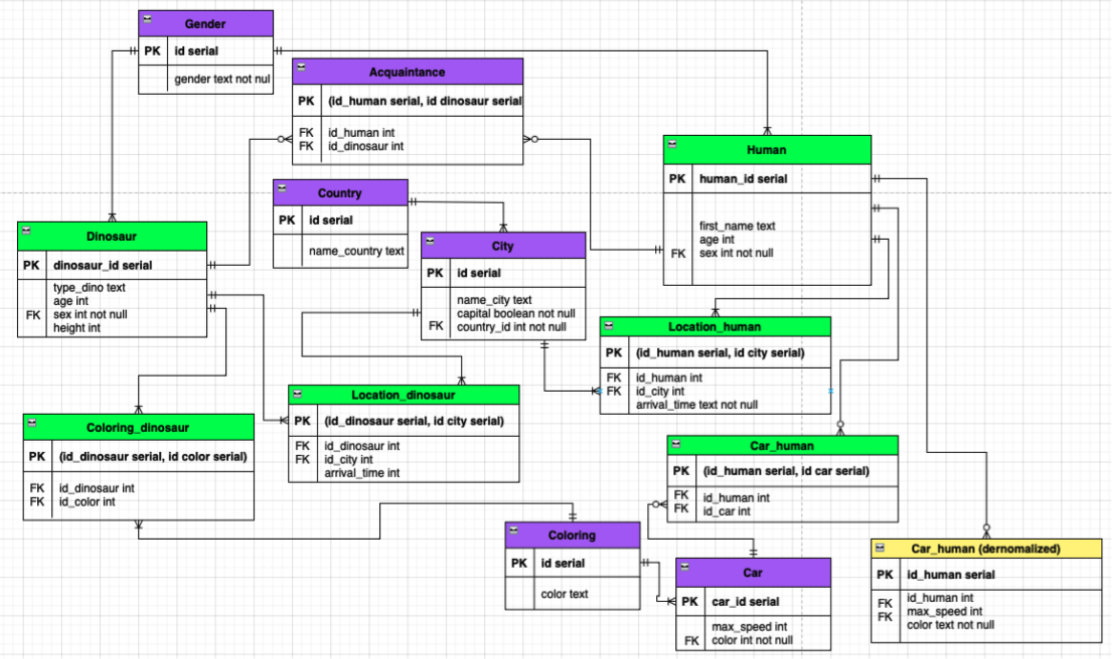
\includegraphics[width=.9\textwidth]{123}